\scalebox{0.9}{
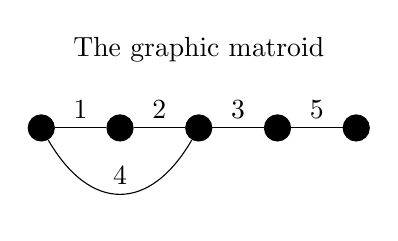
\begin{tikzpicture}[
    node distance=1cm
]
  \node[circle,draw,fill] (a) {};
  \node[circle,draw,fill,right of=a] (b) {};
  \node[circle,draw,fill,right of=b] (c) {};
  \node[circle,draw,fill,right of=c] (d) {};
  \node[circle,draw,fill,right of=d] (e) {};

  \draw (a) -- node[above] {1} (b);
  \draw (b) -- node[above] {2} (c);
  \draw (c) -- node[above] {3} (d);
  \draw (d) -- node[above] {5} (e);
  \draw (a) edge[bend right=60,looseness=1.5] node[above] {4} (c);
  
  \node[above of=c] {\normalsize The graphic matroid};
\end{tikzpicture}
}